\section{Ordenación elemental}
El problema de ordenar un conjunto de elementos es uno de los problemas más estudiados en la historia de la computación. Existen numerosos algoritmos para resolver este problema, cada uno con sus propias características y desventajas. En esta sección estudiaremos el algoritmo de ordenación más sencillo (pero no el más rápido), cuyo procedimiento es el siguiente:

\begin{enumerate}
    \item \textbf{Selecciona} el menor de todos, lo intercambia con el elemento que se encuentra en la primera posición.
    \item \textbf{Selecciona} el menor de los restantes, lo intercambia con el elemento que se encuentra en la segunda posición. 
    \item \textbf{Selecciona} el menor de los restantes, lo intercambia con el elemento que se encuentra en la tercera posición. 
    \item ... y así sucesivamente hasta que el conjunto esté ordenado.  
\end{enumerate}
\newpage
\subsection{Recurso gráfico}
Para ilustrar el funcionamiento del algoritmo de ordenación por selección, se ha desarrollado un recurso gráfico que permite visualizar el estado del conjunto en cada iteración. Supongamos que se tiene la lista:
\begin{equation*}
    [ \ 3,44,38,5,40 \ ]
\end{equation*}
y lo que se busca es aplicar el algoritmo de ordenación por selección.

\textbf{Paso 1:} Se fija la primera posición:

\begin{figure}[h!]  
    \centering
    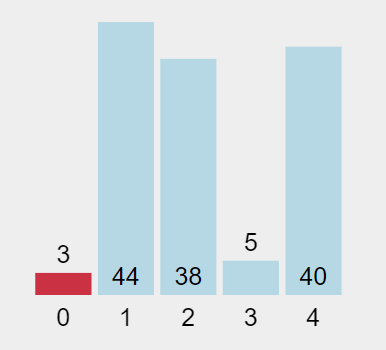
\includegraphics[width=0.5\textwidth]{./Images/oe1.png}
    \caption{Paso 1 del algoritmo de ordenación por selección.}
    \label{fig:SelectionSort1}
\end{figure}

\textbf{Paso 2:} Se busca un número menor que 3, no se encuentra, por lo que no se intercambia nada.

\begin{figure}[h!]  
    \centering
    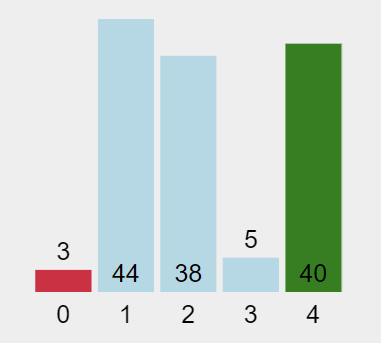
\includegraphics[width=0.5\textwidth]{./Images/oe2.png}
    \caption{Paso 2 del algoritmo de ordenación por selección.}
    \label{fig:SelectionSort2}
\end{figure}

\newpage
\textbf{Paso 3:} Se fija la segunda posición, el color amarillo significa que el número ya está ordenado.

\begin{figure}[h!]  
    \centering
    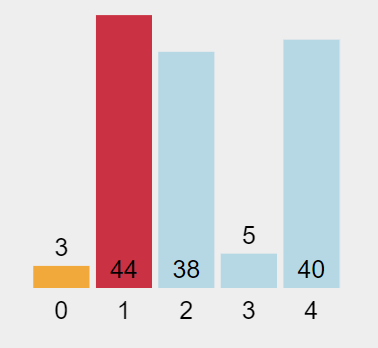
\includegraphics[width=0.5\textwidth]{./Images/oe3.png}
    \caption{Paso 3 del algoritmo de ordenación por selección.}
    \label{fig:SelectionSort3}
\end{figure}

\textbf{Paso 4:} Se busca un número menor que 44, luego uno menor que el menor que haya encontrado que es el 38, se encuentra el 5, por lo que se intercambian.

\begin{figure}[h!]  
    \centering
    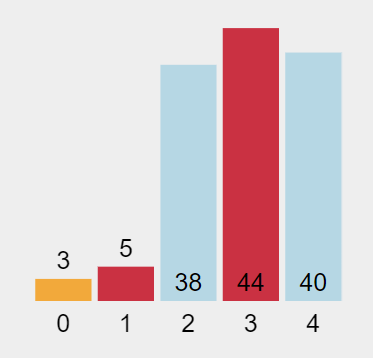
\includegraphics[width=0.5\textwidth]{./Images/oe4.png}
    \caption{Paso 4 del algoritmo de ordenación por selección.}
    \label{fig:SelectionSort4}
\end{figure}

\newpage
\textbf{Paso 5:} Se fija la tercera posición.

\begin{figure}[h!]  
    \centering
    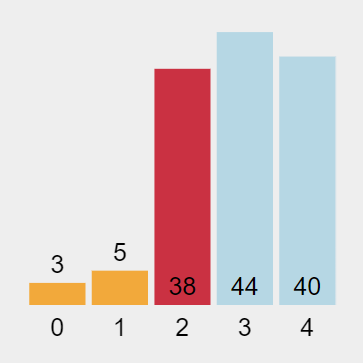
\includegraphics[width=0.5\textwidth]{./Images/oe5.png}
    \caption{Paso 5 del algoritmo de ordenación por selección.}
    \label{fig:SelectionSort5}
\end{figure}

\textbf{Paso 6:} Se busca un número menor que 38, no encuentra ninguno, por lo que no se intercambia nada.

\begin{figure}[h!]  
    \centering
    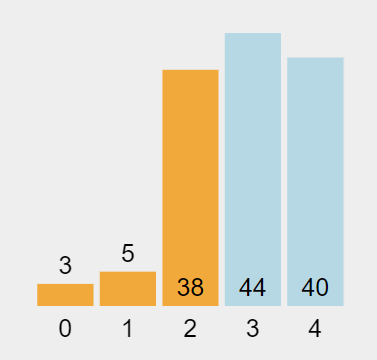
\includegraphics[width=0.5\textwidth]{./Images/oe6.png}
    \caption{Paso 6 del algoritmo de ordenación por selección.}
    \label{fig:SelectionSort6}
\end{figure}

\newpage
\textbf{Paso 7:} Se fija la cuarta posición.

\begin{figure}[h!]  
    \centering
    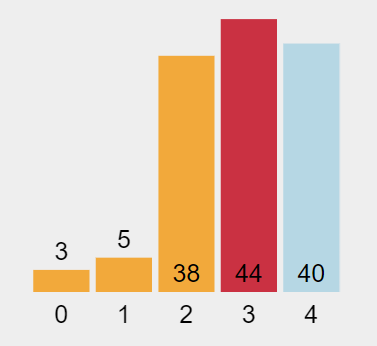
\includegraphics[width=0.5\textwidth]{./Images/oe7.png}
    \caption{Paso 7 del algoritmo de ordenación por selección.}
    \label{fig:SelectionSort7}
\end{figure}

\textbf{Paso 8:} Se busca un número menor a 44, encuentra el 40, por lo que se intercambian.

\begin{figure}[h!]  
    \centering
    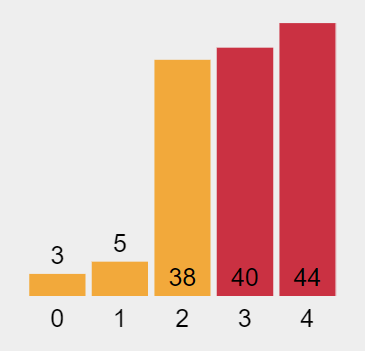
\includegraphics[width=0.5\textwidth]{./Images/oe8.png}
    \caption{Paso 8 del algoritmo de ordenación por selección.}
    \label{fig:SelectionSort8}
\end{figure}

\newpage
\textbf{Final}, el arreglo queda ordenado.

\begin{figure}[h!]  
    \centering
    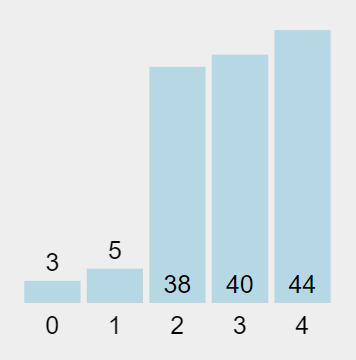
\includegraphics[width=0.5\textwidth]{./Images/oe9.png}
    \caption{Paso 9 del algoritmo de ordenación por selección.}
    \label{fig:SelectionSort9}
\end{figure}

\subsection{Código}

\begin{pascallike}
proc selection_sort (in/out a: array[1..n] of T)
    var minp: nat
    for i := 1 to n do
        minp := min_pos_from(a, i)
        swap(a, i, minp) 
    od
end proc

fun min_pos_from (a: array[1..n] of T, i: nat) ret minp: nat
    minp := i
    for j:= i+1 to n do 
        if a[j] < a[minp] then 
            minp:= j 
        fi
    od
end fun

proc swap (in/out a: array[1..n] of T, in i, j: nat)
    var temp: T
    temp := a[i]
    a[i] := a[j]
    a[j] := temp
end proc
\end{pascallike}

Para el algoritmo de ordenación por selección, se ha desarrollado un procedimiento \texttt{selection\_sort} que recibe un arreglo de tamaño $n$ y lo ordena. El procedimiento \texttt{selection\_sort} utiliza dos funciones auxiliares: \texttt{min\_pos\_from} y \texttt{swap}. La función \texttt{min\_pos\_from} recibe un arreglo y una posición, y retorna la posición del menor elemento a partir de la posición dada. La función \texttt{swap} recibe un arreglo y dos posiciones, e intercambia los elementos en dichas posiciones. 